\documentclass[1p]{elsarticle_modified}
%\bibliographystyle{elsarticle-num}

%\usepackage[colorlinks]{hyperref}
%\usepackage{abbrmath_seonhwa} %\Abb, \Ascr, \Acal ,\Abf, \Afrak
\usepackage{amsfonts}
\usepackage{amssymb}
\usepackage{amsmath}
\usepackage{amsthm}
\usepackage{scalefnt}
\usepackage{amsbsy}
\usepackage{kotex}
\usepackage{caption}
\usepackage{subfig}
\usepackage{color}
\usepackage{graphicx}
\usepackage{xcolor} %% white, black, red, green, blue, cyan, magenta, yellow
\usepackage{float}
\usepackage{setspace}
\usepackage{hyperref}

\usepackage{tikz}
\usetikzlibrary{arrows}

\usepackage{multirow}
\usepackage{array} % fixed length table
\usepackage{hhline}

%%%%%%%%%%%%%%%%%%%%%
\makeatletter
\renewcommand*\env@matrix[1][\arraystretch]{%
	\edef\arraystretch{#1}%
	\hskip -\arraycolsep
	\let\@ifnextchar\new@ifnextchar
	\array{*\c@MaxMatrixCols c}}
\makeatother %https://tex.stackexchange.com/questions/14071/how-can-i-increase-the-line-spacing-in-a-matrix
%%%%%%%%%%%%%%%

\usepackage[normalem]{ulem}

\newcommand{\msout}[1]{\ifmmode\text{\sout{\ensuremath{#1}}}\else\sout{#1}\fi}
%SOURCE: \msout is \stkout macro in https://tex.stackexchange.com/questions/20609/strikeout-in-math-mode

\newcommand{\cancel}[1]{
	\ifmmode
	{\color{red}\msout{#1}}
	\else
	{\color{red}\sout{#1}}
	\fi
}

\newcommand{\add}[1]{
	{\color{blue}\uwave{#1}}
}

\newcommand{\replace}[2]{
	\ifmmode
	{\color{red}\msout{#1}}{\color{blue}\uwave{#2}}
	\else
	{\color{red}\sout{#1}}{\color{blue}\uwave{#2}}
	\fi
}

\newcommand{\Sol}{\mathcal{S}} %segment
\newcommand{\D}{D} %diagram
\newcommand{\A}{\mathcal{A}} %arc


%%%%%%%%%%%%%%%%%%%%%%%%%%%%%5 test

\def\sl{\operatorname{\textup{SL}}(2,\Cbb)}
\def\psl{\operatorname{\textup{PSL}}(2,\Cbb)}
\def\quan{\mkern 1mu \triangleright \mkern 1mu}

\theoremstyle{definition}
\newtheorem{thm}{Theorem}[section]
\newtheorem{prop}[thm]{Proposition}
\newtheorem{lem}[thm]{Lemma}
\newtheorem{ques}[thm]{Question}
\newtheorem{cor}[thm]{Corollary}
\newtheorem{defn}[thm]{Definition}
\newtheorem{exam}[thm]{Example}
\newtheorem{rmk}[thm]{Remark}
\newtheorem{alg}[thm]{Algorithm}

\newcommand{\I}{\sqrt{-1}}
\begin{document}

%\begin{frontmatter}
%
%\title{Boundary parabolic representations of knots up to 8 crossings}
%
%%% Group authors per affiliation:
%\author{Yunhi Cho} 
%\address{Department of Mathematics, University of Seoul, Seoul, Korea}
%\ead{yhcho@uos.ac.kr}
%
%
%\author{Seonhwa Kim} %\fnref{s_kim}}
%\address{Center for Geometry and Physics, Institute for Basic Science, Pohang, 37673, Korea}
%\ead{ryeona17@ibs.re.kr}
%
%\author{Hyuk Kim}
%\address{Department of Mathematical Sciences, Seoul National University, Seoul 08826, Korea}
%\ead{hyukkim@snu.ac.kr}
%
%\author{Seokbeom Yoon}
%\address{Department of Mathematical Sciences, Seoul National University, Seoul, 08826,  Korea}
%\ead{sbyoon15@snu.ac.kr}
%
%\begin{abstract}
%We find all boundary parabolic representation of knots up to 8 crossings.
%
%\end{abstract}
%\begin{keyword}
%    \MSC[2010] 57M25 
%\end{keyword}
%
%\end{frontmatter}

%\linenumbers
%\tableofcontents
%
\newcommand\colored[1]{\textcolor{white}{\rule[-0.35ex]{0.8em}{1.4ex}}\kern-0.8em\color{red} #1}%
%\newcommand\colored[1]{\textcolor{white}{ #1}\kern-2.17ex	\textcolor{white}{ #1}\kern-1.81ex	\textcolor{white}{ #1}\kern-2.15ex\color{red}#1	}

{\Large $\underline{12n_{0405}~(K12n_{0405})}$}

\setlength{\tabcolsep}{10pt}
\renewcommand{\arraystretch}{1.6}
\vspace{1cm}\begin{tabular}{m{100pt}>{\centering\arraybackslash}m{274pt}}
\multirow{5}{120pt}{
	\centering
	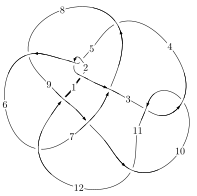
\includegraphics[width=112pt]{../../../GIT/diagram.site/Diagrams/png/2494_12n_0405.png}\\
\ \ \ A knot diagram\footnotemark}&
\allowdisplaybreaks
\textbf{Linearized knot diagam} \\
\cline{2-2}
 &
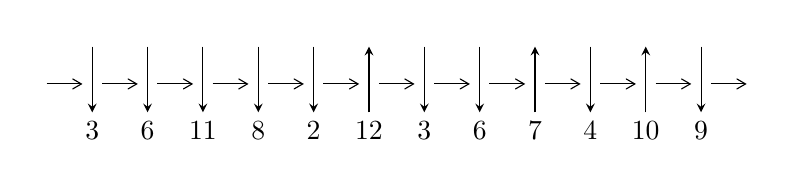
\begin{tikzpicture}[x=20pt, y=17pt]
	% nodes
	\node (C0) at (0, 0) {};
	\node (C1) at (1, 0) {};
	\node (C1U) at (1, +1) {};
	\node (C1D) at (1, -1) {3};

	\node (C2) at (2, 0) {};
	\node (C2U) at (2, +1) {};
	\node (C2D) at (2, -1) {6};

	\node (C3) at (3, 0) {};
	\node (C3U) at (3, +1) {};
	\node (C3D) at (3, -1) {11};

	\node (C4) at (4, 0) {};
	\node (C4U) at (4, +1) {};
	\node (C4D) at (4, -1) {8};

	\node (C5) at (5, 0) {};
	\node (C5U) at (5, +1) {};
	\node (C5D) at (5, -1) {2};

	\node (C6) at (6, 0) {};
	\node (C6U) at (6, +1) {};
	\node (C6D) at (6, -1) {12};

	\node (C7) at (7, 0) {};
	\node (C7U) at (7, +1) {};
	\node (C7D) at (7, -1) {3};

	\node (C8) at (8, 0) {};
	\node (C8U) at (8, +1) {};
	\node (C8D) at (8, -1) {6};

	\node (C9) at (9, 0) {};
	\node (C9U) at (9, +1) {};
	\node (C9D) at (9, -1) {7};

	\node (C10) at (10, 0) {};
	\node (C10U) at (10, +1) {};
	\node (C10D) at (10, -1) {4};

	\node (C11) at (11, 0) {};
	\node (C11U) at (11, +1) {};
	\node (C11D) at (11, -1) {10};

	\node (C12) at (12, 0) {};
	\node (C12U) at (12, +1) {};
	\node (C12D) at (12, -1) {9};
	\node (C13) at (13, 0) {};

	% arrows
	\draw[->,>={angle 60}]
	(C0) edge (C1) (C1) edge (C2) (C2) edge (C3) (C3) edge (C4) (C4) edge (C5) (C5) edge (C6) (C6) edge (C7) (C7) edge (C8) (C8) edge (C9) (C9) edge (C10) (C10) edge (C11) (C11) edge (C12) (C12) edge (C13) ;	\draw[->,>=stealth]
	(C1U) edge (C1D) (C2U) edge (C2D) (C3U) edge (C3D) (C4U) edge (C4D) (C5U) edge (C5D) (C6D) edge (C6U) (C7U) edge (C7D) (C8U) edge (C8D) (C9D) edge (C9U) (C10U) edge (C10D) (C11D) edge (C11U) (C12U) edge (C12D) ;
	\end{tikzpicture} \\
\hhline{~~} \\& 
\textbf{Solving Sequence} \\ \cline{2-2} 
 &
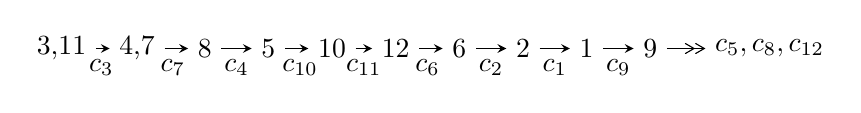
\begin{tikzpicture}[x=23pt, y=7pt]
	% node
	\node (A0) at (-1/8, 0) {3,11};
	\node (A1) at (17/16, 0) {4,7};
	\node (A2) at (17/8, 0) {8};
	\node (A3) at (25/8, 0) {5};
	\node (A4) at (33/8, 0) {10};
	\node (A5) at (41/8, 0) {12};
	\node (A6) at (49/8, 0) {6};
	\node (A7) at (57/8, 0) {2};
	\node (A8) at (65/8, 0) {1};
	\node (A9) at (73/8, 0) {9};
	\node (C1) at (1/2, -1) {$c_{3}$};
	\node (C2) at (13/8, -1) {$c_{7}$};
	\node (C3) at (21/8, -1) {$c_{4}$};
	\node (C4) at (29/8, -1) {$c_{10}$};
	\node (C5) at (37/8, -1) {$c_{11}$};
	\node (C6) at (45/8, -1) {$c_{6}$};
	\node (C7) at (53/8, -1) {$c_{2}$};
	\node (C8) at (61/8, -1) {$c_{1}$};
	\node (C9) at (69/8, -1) {$c_{9}$};
	\node (A10) at (11, 0) {$c_{5},c_{8},c_{12}$};

	% edge
	\draw[->,>=stealth]	
	(A0) edge (A1) (A1) edge (A2) (A2) edge (A3) (A3) edge (A4) (A4) edge (A5) (A5) edge (A6) (A6) edge (A7) (A7) edge (A8) (A8) edge (A9) ;
	\draw[->>,>={angle 60}]	
	(A9) edge (A10);
\end{tikzpicture} \\ 

\end{tabular} \\

\footnotetext{
The image of knot diagram is generated by the software ``\textbf{Draw programme}" developed by Andrew Bartholomew(\url{http://www.layer8.co.uk/maths/draw/index.htm\#Running-draw}), where we modified some parts for our purpose(\url{https://github.com/CATsTAILs/LinksPainter}).
}\phantom \\ \newline 
\centering \textbf{Ideals for irreducible components\footnotemark of $X_{\text{par}}$} 
 
\begin{align*}
I^u_{1}&=\langle 
-5.04740\times10^{30} u^{55}-2.66361\times10^{30} u^{54}+\cdots+5.37736\times10^{30} b-1.62190\times10^{31},\\
\phantom{I^u_{1}}&\phantom{= \langle  }-1.29311\times10^{31} u^{55}-2.08861\times10^{29} u^{54}+\cdots+1.07547\times10^{31} a+7.57948\times10^{31},\;u^{56}+u^{55}+\cdots+11 u+1\rangle \\
I^u_{2}&=\langle 
- u^{18}-5 u^{16}+\cdots+b-1,\;-39 u^{19}-13 u^{18}+\cdots+46 a-113,\;u^{20}+5 u^{18}+\cdots+3 u+1\rangle \\
\\
\end{align*}
\raggedright * 2 irreducible components of $\dim_{\mathbb{C}}=0$, with total 76 representations.\\
\footnotetext{All coefficients of polynomials are rational numbers. But the coefficients are sometimes approximated in decimal forms when there is not enough margin.}
\newpage
\renewcommand{\arraystretch}{1}
\centering \section*{I. $I^u_{1}= \langle -5.05\times10^{30} u^{55}-2.66\times10^{30} u^{54}+\cdots+5.38\times10^{30} b-1.62\times10^{31},\;-1.29\times10^{31} u^{55}-2.09\times10^{29} u^{54}+\cdots+1.08\times10^{31} a+7.58\times10^{31},\;u^{56}+u^{55}+\cdots+11 u+1 \rangle$}
\flushleft \textbf{(i) Arc colorings}\\
\begin{tabular}{m{7pt} m{180pt} m{7pt} m{180pt} }
\flushright $a_{3}=$&$\begin{pmatrix}1\\0\end{pmatrix}$ \\
\flushright $a_{11}=$&$\begin{pmatrix}0\\u\end{pmatrix}$ \\
\flushright $a_{4}=$&$\begin{pmatrix}1\\u^2\end{pmatrix}$ \\
\flushright $a_{7}=$&$\begin{pmatrix}1.20236 u^{55}+0.0194204 u^{54}+\cdots+2.12491 u-7.04759\\0.938638 u^{55}+0.495339 u^{54}+\cdots+12.7233 u+3.01616\end{pmatrix}$ \\
\flushright $a_{8}=$&$\begin{pmatrix}0.263723 u^{55}-0.475918 u^{54}+\cdots-10.5984 u-10.0637\\0.938638 u^{55}+0.495339 u^{54}+\cdots+12.7233 u+3.01616\end{pmatrix}$ \\
\flushright $a_{5}=$&$\begin{pmatrix}-1.47729 u^{55}-2.00842 u^{54}+\cdots-77.8992 u-24.8854\\1.30201 u^{55}+0.374284 u^{54}+\cdots+17.0385 u+5.14052\end{pmatrix}$ \\
\flushright $a_{10}=$&$\begin{pmatrix}u\\u^3+u\end{pmatrix}$ \\
\flushright $a_{12}=$&$\begin{pmatrix}u^3\\u^5+u^3+u\end{pmatrix}$ \\
\flushright $a_{6}=$&$\begin{pmatrix}1.26914 u^{55}-0.0878330 u^{54}+\cdots+2.68555 u-7.01937\\0.932246 u^{55}+0.339280 u^{54}+\cdots+7.82652 u+2.41420\end{pmatrix}$ \\
\flushright $a_{2}=$&$\begin{pmatrix}-0.0113393 u^{55}+0.701676 u^{54}+\cdots+33.7128 u+17.2063\\-0.985020 u^{55}+0.0619797 u^{54}+\cdots-14.0951 u-4.29081\end{pmatrix}$ \\
\flushright $a_{1}=$&$\begin{pmatrix}-0.996359 u^{55}+0.763656 u^{54}+\cdots+19.6177 u+12.9155\\-0.985020 u^{55}+0.0619797 u^{54}+\cdots-14.0951 u-4.29081\end{pmatrix}$ \\
\flushright $a_{9}=$&$\begin{pmatrix}-0.673812 u^{55}+1.74584 u^{54}+\cdots+30.9969 u+11.4293\\-1.53887 u^{55}-0.462506 u^{54}+\cdots-10.8493 u-3.21916\end{pmatrix}$\\&\end{tabular}
\flushleft \textbf{(ii) Obstruction class $= -1$}\\~\\
\flushleft \textbf{(iii) Cusp Shapes $= -3.20118 u^{55}-1.25466 u^{54}+\cdots-55.5550 u-11.0853$}\\~\\
\newpage\renewcommand{\arraystretch}{1}
\flushleft \textbf{(iv) u-Polynomials at the component}\newline \\
\begin{tabular}{m{50pt}|m{274pt}}
Crossings & \hspace{64pt}u-Polynomials at each crossing \\
\hline $$\begin{aligned}c_{1}\end{aligned}$$&$\begin{aligned}
&u^{56}+81 u^{55}+\cdots-82 u+1
\end{aligned}$\\
\hline $$\begin{aligned}c_{2},c_{5}\end{aligned}$$&$\begin{aligned}
&u^{56}+3 u^{55}+\cdots+20 u-1
\end{aligned}$\\
\hline $$\begin{aligned}c_{3},c_{10}\end{aligned}$$&$\begin{aligned}
&u^{56}+u^{55}+\cdots+11 u+1
\end{aligned}$\\
\hline $$\begin{aligned}c_{4}\end{aligned}$$&$\begin{aligned}
&u^{56}- u^{55}+\cdots-5248 u-1021
\end{aligned}$\\
\hline $$\begin{aligned}c_{6}\end{aligned}$$&$\begin{aligned}
&u^{56}-2 u^{55}+\cdots+74 u+127
\end{aligned}$\\
\hline $$\begin{aligned}c_{7}\end{aligned}$$&$\begin{aligned}
&u^{56}- u^{55}+\cdots+211173 u-7921
\end{aligned}$\\
\hline $$\begin{aligned}c_{8}\end{aligned}$$&$\begin{aligned}
&u^{56}+10 u^{55}+\cdots+155830 u+215404
\end{aligned}$\\
\hline $$\begin{aligned}c_{9}\end{aligned}$$&$\begin{aligned}
&u^{56}+16 u^{55}+\cdots+815 u+53
\end{aligned}$\\
\hline $$\begin{aligned}c_{11}\end{aligned}$$&$\begin{aligned}
&u^{56}-23 u^{55}+\cdots+43 u+1
\end{aligned}$\\
\hline $$\begin{aligned}c_{12}\end{aligned}$$&$\begin{aligned}
&u^{56}-9 u^{55}+\cdots-735411 u-85511
\end{aligned}$\\
\hline
\end{tabular}\\~\\
\newpage\renewcommand{\arraystretch}{1}
\flushleft \textbf{(v) Riley Polynomials at the component}\newline \\
\begin{tabular}{m{50pt}|m{274pt}}
Crossings & \hspace{64pt}Riley Polynomials at each crossing \\
\hline $$\begin{aligned}c_{1}\end{aligned}$$&$\begin{aligned}
&y^{56}-201 y^{55}+\cdots-18994 y+1
\end{aligned}$\\
\hline $$\begin{aligned}c_{2},c_{5}\end{aligned}$$&$\begin{aligned}
&y^{56}-81 y^{55}+\cdots+82 y+1
\end{aligned}$\\
\hline $$\begin{aligned}c_{3},c_{10}\end{aligned}$$&$\begin{aligned}
&y^{56}+23 y^{55}+\cdots-43 y+1
\end{aligned}$\\
\hline $$\begin{aligned}c_{4}\end{aligned}$$&$\begin{aligned}
&y^{56}-97 y^{55}+\cdots+134121594 y+1042441
\end{aligned}$\\
\hline $$\begin{aligned}c_{6}\end{aligned}$$&$\begin{aligned}
&y^{56}+14 y^{55}+\cdots+197216 y+16129
\end{aligned}$\\
\hline $$\begin{aligned}c_{7}\end{aligned}$$&$\begin{aligned}
&y^{56}-59 y^{55}+\cdots+2248587717 y+62742241
\end{aligned}$\\
\hline $$\begin{aligned}c_{8}\end{aligned}$$&$\begin{aligned}
&y^{56}-106 y^{55}+\cdots-2285891007612 y+46398883216
\end{aligned}$\\
\hline $$\begin{aligned}c_{9}\end{aligned}$$&$\begin{aligned}
&y^{56}+12 y^{55}+\cdots-7449 y+2809
\end{aligned}$\\
\hline $$\begin{aligned}c_{11}\end{aligned}$$&$\begin{aligned}
&y^{56}+27 y^{55}+\cdots-3871 y+1
\end{aligned}$\\
\hline $$\begin{aligned}c_{12}\end{aligned}$$&$\begin{aligned}
&y^{56}-45 y^{55}+\cdots-1207444021181 y+7312131121
\end{aligned}$\\
\hline
\end{tabular}\\~\\
\newpage\flushleft \textbf{(vi) Complex Volumes and Cusp Shapes}
$$\begin{array}{c|c|c}  
\text{Solutions to }I^u_{1}& \I (\text{vol} + \sqrt{-1}CS) & \text{Cusp shape}\\
 \hline 
\begin{aligned}
u &= \phantom{-}0.692976 + 0.741456 I \\
a &= \phantom{-}0.83415 - 2.68568 I \\
b &= \phantom{-}2.82225 - 1.87057 I\end{aligned}
 & -13.01880 - 0.11658 I & -13.39749 + 0.26224 I \\ \hline\begin{aligned}
u &= \phantom{-}0.692976 - 0.741456 I \\
a &= \phantom{-}0.83415 + 2.68568 I \\
b &= \phantom{-}2.82225 + 1.87057 I\end{aligned}
 & -13.01880 + 0.11658 I & -13.39749 - 0.26224 I \\ \hline\begin{aligned}
u &= -0.888534 + 0.493154 I \\
a &= \phantom{-}0.787487 + 0.456037 I \\
b &= \phantom{-}0.828874 + 0.814475 I\end{aligned}
 & -4.23499 - 0.34965 I & -13.31370 + 0. I\phantom{ +0.000000I} \\ \hline\begin{aligned}
u &= -0.888534 - 0.493154 I \\
a &= \phantom{-}0.787487 - 0.456037 I \\
b &= \phantom{-}0.828874 - 0.814475 I\end{aligned}
 & -4.23499 + 0.34965 I & -13.31370 + 0. I\phantom{ +0.000000I} \\ \hline\begin{aligned}
u &= -0.633685 + 0.804537 I \\
a &= \phantom{-}2.26499 + 1.02925 I \\
b &= \phantom{-}1.64637 - 1.29628 I\end{aligned}
 & -2.67621 + 0.18944 I & -11.22703 - 1.60949 I \\ \hline\begin{aligned}
u &= -0.633685 - 0.804537 I \\
a &= \phantom{-}2.26499 - 1.02925 I \\
b &= \phantom{-}1.64637 + 1.29628 I\end{aligned}
 & -2.67621 - 0.18944 I & -11.22703 + 1.60949 I \\ \hline\begin{aligned}
u &= -0.633438 + 0.738930 I \\
a &= \phantom{-}1.67728 - 0.91484 I \\
b &= \phantom{-}1.368790 + 0.135930 I\end{aligned}
 & -12.20520 + 0.71501 I & -16.2418 + 1.0323 I \\ \hline\begin{aligned}
u &= -0.633438 - 0.738930 I \\
a &= \phantom{-}1.67728 + 0.91484 I \\
b &= \phantom{-}1.368790 - 0.135930 I\end{aligned}
 & -12.20520 - 0.71501 I & -16.2418 - 1.0323 I \\ \hline\begin{aligned}
u &= \phantom{-}0.858766 + 0.568486 I \\
a &= \phantom{-}1.39718 - 0.43816 I \\
b &= \phantom{-}1.51683 + 0.16349 I\end{aligned}
 & -4.83444 + 3.81788 I & -12.17523 - 2.36589 I \\ \hline\begin{aligned}
u &= \phantom{-}0.858766 - 0.568486 I \\
a &= \phantom{-}1.39718 + 0.43816 I \\
b &= \phantom{-}1.51683 - 0.16349 I\end{aligned}
 & -4.83444 - 3.81788 I & -12.17523 + 2.36589 I\\
 \hline 
 \end{array}$$\newpage$$\begin{array}{c|c|c}  
\text{Solutions to }I^u_{1}& \I (\text{vol} + \sqrt{-1}CS) & \text{Cusp shape}\\
 \hline 
\begin{aligned}
u &= \phantom{-}0.636578 + 0.817575 I \\
a &= -0.793907 + 0.325846 I \\
b &= -0.824038 + 0.535982 I\end{aligned}
 & -3.51130 - 0.72418 I & -12.99804 - 0.44886 I \\ \hline\begin{aligned}
u &= \phantom{-}0.636578 - 0.817575 I \\
a &= -0.793907 - 0.325846 I \\
b &= -0.824038 - 0.535982 I\end{aligned}
 & -3.51130 + 0.72418 I & -12.99804 + 0.44886 I \\ \hline\begin{aligned}
u &= \phantom{-}0.104993 + 1.060980 I \\
a &= \phantom{-}0.053924 + 0.614830 I \\
b &= \phantom{-}0.345359 - 0.952663 I\end{aligned}
 & \phantom{-}3.62265 + 0.91650 I & \phantom{-}                -6
0.912924 + 0. 10   I\phantom{ +0.000000I} \\ \hline\begin{aligned}
u &= \phantom{-}0.104993 - 1.060980 I \\
a &= \phantom{-}0.053924 - 0.614830 I \\
b &= \phantom{-}0.345359 + 0.952663 I\end{aligned}
 & \phantom{-}3.62265 - 0.91650 I & \phantom{-}                -6
0.912924 + 0. 10   I\phantom{ +0.000000I} \\ \hline\begin{aligned}
u &= -0.047680 + 0.929101 I \\
a &= \phantom{-}2.35142 - 0.07585 I \\
b &= -0.959476 + 0.938322 I\end{aligned}
 & -8.23805 + 0.54981 I & -5.62601 + 0.13195 I \\ \hline\begin{aligned}
u &= -0.047680 - 0.929101 I \\
a &= \phantom{-}2.35142 + 0.07585 I \\
b &= -0.959476 - 0.938322 I\end{aligned}
 & -8.23805 - 0.54981 I & -5.62601 - 0.13195 I \\ \hline\begin{aligned}
u &= \phantom{-}0.639057 + 0.870621 I \\
a &= \phantom{-}1.25596 - 0.86121 I \\
b &= \phantom{-}0.544969 + 0.721077 I\end{aligned}
 & -3.35127 - 4.26074 I & -12.1347 + 7.9623 I \\ \hline\begin{aligned}
u &= \phantom{-}0.639057 - 0.870621 I \\
a &= \phantom{-}1.25596 + 0.86121 I \\
b &= \phantom{-}0.544969 - 0.721077 I\end{aligned}
 & -3.35127 + 4.26074 I & -12.1347 - 7.9623 I \\ \hline\begin{aligned}
u &= -0.622311 + 0.676205 I \\
a &= -1.52391 + 0.07731 I \\
b &= -0.701853 + 0.906118 I\end{aligned}
 & -1.41377 + 1.41882 I & -7.66827 - 2.37637 I \\ \hline\begin{aligned}
u &= -0.622311 - 0.676205 I \\
a &= -1.52391 - 0.07731 I \\
b &= -0.701853 - 0.906118 I\end{aligned}
 & -1.41377 - 1.41882 I & -7.66827 + 2.37637 I\\
 \hline 
 \end{array}$$\newpage$$\begin{array}{c|c|c}  
\text{Solutions to }I^u_{1}& \I (\text{vol} + \sqrt{-1}CS) & \text{Cusp shape}\\
 \hline 
\begin{aligned}
u &= \phantom{-}1.002470 + 0.434054 I \\
a &= -0.995062 - 0.161033 I \\
b &= -1.65678 - 0.10063 I\end{aligned}
 & -14.5702 - 3.5038 I & -12.90961 + 3.29634 I \\ \hline\begin{aligned}
u &= \phantom{-}1.002470 - 0.434054 I \\
a &= -0.995062 + 0.161033 I \\
b &= -1.65678 + 0.10063 I\end{aligned}
 & -14.5702 + 3.5038 I & -12.90961 - 3.29634 I \\ \hline\begin{aligned}
u &= -0.934670 + 0.567956 I \\
a &= -1.31747 - 1.19240 I \\
b &= -1.95969 - 1.15142 I\end{aligned}
 & -15.5375 - 8.7539 I & -11.13073 + 3.10208 I \\ \hline\begin{aligned}
u &= -0.934670 - 0.567956 I \\
a &= -1.31747 + 1.19240 I \\
b &= -1.95969 + 1.15142 I\end{aligned}
 & -15.5375 + 8.7539 I & -11.13073 - 3.10208 I \\ \hline\begin{aligned}
u &= -0.631753 + 0.901368 I \\
a &= -1.02898 - 1.61492 I \\
b &= -2.09741 - 0.75187 I\end{aligned}
 & -2.37070 + 4.76407 I & -10.20100 - 5.68692 I \\ \hline\begin{aligned}
u &= -0.631753 - 0.901368 I \\
a &= -1.02898 + 1.61492 I \\
b &= -2.09741 + 0.75187 I\end{aligned}
 & -2.37070 - 4.76407 I & -10.20100 + 5.68692 I \\ \hline\begin{aligned}
u &= -0.204920 + 1.113530 I \\
a &= \phantom{-}0.265324 + 0.432938 I \\
b &= \phantom{-}0.0303195 + 0.0315283 I\end{aligned}
 & \phantom{-}2.10184 + 2.44163 I & -6.00000 - 6.66179 I \\ \hline\begin{aligned}
u &= -0.204920 - 1.113530 I \\
a &= \phantom{-}0.265324 - 0.432938 I \\
b &= \phantom{-}0.0303195 - 0.0315283 I\end{aligned}
 & \phantom{-}2.10184 - 2.44163 I & -6.00000 + 6.66179 I \\ \hline\begin{aligned}
u &= -0.637975 + 0.945501 I \\
a &= -0.49971 - 2.41919 I \\
b &= -1.051990 + 0.178832 I\end{aligned}
 & -11.56320 + 4.27962 I & \phantom{-0.000000 } 0 \\ \hline\begin{aligned}
u &= -0.637975 - 0.945501 I \\
a &= -0.49971 + 2.41919 I \\
b &= -1.051990 - 0.178832 I\end{aligned}
 & -11.56320 - 4.27962 I & \phantom{-0.000000 } 0\\
 \hline 
 \end{array}$$\newpage$$\begin{array}{c|c|c}  
\text{Solutions to }I^u_{1}& \I (\text{vol} + \sqrt{-1}CS) & \text{Cusp shape}\\
 \hline 
\begin{aligned}
u &= \phantom{-}0.628401 + 0.578258 I \\
a &= -1.49132 + 0.91673 I \\
b &= -0.663752 + 0.368778 I\end{aligned}
 & -0.88901 + 2.15046 I & -6.68954 - 4.21266 I \\ \hline\begin{aligned}
u &= \phantom{-}0.628401 - 0.578258 I \\
a &= -1.49132 - 0.91673 I \\
b &= -0.663752 - 0.368778 I\end{aligned}
 & -0.88901 - 2.15046 I & -6.68954 + 4.21266 I \\ \hline\begin{aligned}
u &= -0.617638 + 0.982030 I \\
a &= \phantom{-}0.453503 + 0.970711 I \\
b &= \phantom{-}1.147700 + 0.399179 I\end{aligned}
 & -0.48219 + 3.48780 I & \phantom{-0.000000 } 0 \\ \hline\begin{aligned}
u &= -0.617638 - 0.982030 I \\
a &= \phantom{-}0.453503 - 0.970711 I \\
b &= \phantom{-}1.147700 - 0.399179 I\end{aligned}
 & -0.48219 - 3.48780 I & \phantom{-0.000000 } 0 \\ \hline\begin{aligned}
u &= \phantom{-}0.674791 + 0.947519 I \\
a &= -2.87088 + 0.86323 I \\
b &= -2.20281 - 2.50210 I\end{aligned}
 & -12.39390 - 5.16219 I & \phantom{-0.000000 } 0 \\ \hline\begin{aligned}
u &= \phantom{-}0.674791 - 0.947519 I \\
a &= -2.87088 - 0.86323 I \\
b &= -2.20281 + 2.50210 I\end{aligned}
 & -12.39390 + 5.16219 I & \phantom{-0.000000 } 0 \\ \hline\begin{aligned}
u &= -0.205795 + 0.791172 I \\
a &= -0.622285 - 0.611724 I \\
b &= -1.082330 - 0.398478 I\end{aligned}
 & \phantom{-}0.118397 - 0.860000 I & -3.74291 + 1.06399 I \\ \hline\begin{aligned}
u &= -0.205795 - 0.791172 I \\
a &= -0.622285 + 0.611724 I \\
b &= -1.082330 + 0.398478 I\end{aligned}
 & \phantom{-}0.118397 + 0.860000 I & -3.74291 - 1.06399 I \\ \hline\begin{aligned}
u &= \phantom{-}0.622297 + 1.014000 I \\
a &= \phantom{-}1.75434 - 0.58914 I \\
b &= \phantom{-}0.968744 + 0.647144 I\end{aligned}
 & \phantom{-}0.37205 - 7.12007 I & \phantom{-0.000000 } 0 \\ \hline\begin{aligned}
u &= \phantom{-}0.622297 - 1.014000 I \\
a &= \phantom{-}1.75434 + 0.58914 I \\
b &= \phantom{-}0.968744 - 0.647144 I\end{aligned}
 & \phantom{-}0.37205 + 7.12007 I & \phantom{-0.000000 } 0\\
 \hline 
 \end{array}$$\newpage$$\begin{array}{c|c|c}  
\text{Solutions to }I^u_{1}& \I (\text{vol} + \sqrt{-1}CS) & \text{Cusp shape}\\
 \hline 
\begin{aligned}
u &= \phantom{-}0.693949 + 1.070290 I \\
a &= -0.98029 + 1.20357 I \\
b &= -1.74189 - 0.24768 I\end{aligned}
 & -3.32079 - 9.58196 I & \phantom{-0.000000 } 0 \\ \hline\begin{aligned}
u &= \phantom{-}0.693949 - 1.070290 I \\
a &= -0.98029 - 1.20357 I \\
b &= -1.74189 + 0.24768 I\end{aligned}
 & -3.32079 + 9.58196 I & \phantom{-0.000000 } 0 \\ \hline\begin{aligned}
u &= -0.137699 + 1.273350 I \\
a &= \phantom{-}0.353439 + 0.379773 I \\
b &= -0.460194 - 0.278269 I\end{aligned}
 & \phantom{-}2.02092 + 2.34731 I & \phantom{-0.000000 } 0 \\ \hline\begin{aligned}
u &= -0.137699 - 1.273350 I \\
a &= \phantom{-}0.353439 - 0.379773 I \\
b &= -0.460194 + 0.278269 I\end{aligned}
 & \phantom{-}2.02092 - 2.34731 I & \phantom{-0.000000 } 0 \\ \hline\begin{aligned}
u &= \phantom{-}0.105350 + 1.287810 I \\
a &= -0.735406 - 0.340219 I \\
b &= \phantom{-}1.31301 + 0.75117 I\end{aligned}
 & -8.24037 - 6.79326 I & \phantom{-0.000000 } 0 \\ \hline\begin{aligned}
u &= \phantom{-}0.105350 - 1.287810 I \\
a &= -0.735406 + 0.340219 I \\
b &= \phantom{-}1.31301 - 0.75117 I\end{aligned}
 & -8.24037 + 6.79326 I & \phantom{-0.000000 } 0 \\ \hline\begin{aligned}
u &= -0.684933 + 1.102170 I \\
a &= -1.35653 - 0.57109 I \\
b &= -0.746484 + 1.007420 I\end{aligned}
 & -2.41411 + 6.13994 I & \phantom{-0.000000 } 0 \\ \hline\begin{aligned}
u &= -0.684933 - 1.102170 I \\
a &= -1.35653 + 0.57109 I \\
b &= -0.746484 - 1.007420 I\end{aligned}
 & -2.41411 - 6.13994 I & \phantom{-0.000000 } 0 \\ \hline\begin{aligned}
u &= -0.720000 + 1.106020 I \\
a &= \phantom{-}1.91793 + 1.16363 I \\
b &= \phantom{-}1.89543 - 1.46698 I\end{aligned}
 & -13.8786 + 14.8239 I & \phantom{-0.000000 } 0 \\ \hline\begin{aligned}
u &= -0.720000 - 1.106020 I \\
a &= \phantom{-}1.91793 - 1.16363 I \\
b &= \phantom{-}1.89543 + 1.46698 I\end{aligned}
 & -13.8786 - 14.8239 I & \phantom{-0.000000 } 0\\
 \hline 
 \end{array}$$\newpage$$\begin{array}{c|c|c}  
\text{Solutions to }I^u_{1}& \I (\text{vol} + \sqrt{-1}CS) & \text{Cusp shape}\\
 \hline 
\begin{aligned}
u &= \phantom{-}0.705581 + 1.210660 I \\
a &= \phantom{-}0.274806 - 1.197140 I \\
b &= \phantom{-}1.40944 + 0.27613 I\end{aligned}
 & -12.19060 - 2.71913 I & \phantom{-0.000000 } 0 \\ \hline\begin{aligned}
u &= \phantom{-}0.705581 - 1.210660 I \\
a &= \phantom{-}0.274806 + 1.197140 I \\
b &= \phantom{-}1.40944 - 0.27613 I\end{aligned}
 & -12.19060 + 2.71913 I & \phantom{-0.000000 } 0 \\ \hline\begin{aligned}
u &= \phantom{-}0.001183 + 0.423530 I \\
a &= -2.64102 + 1.15828 I \\
b &= \phantom{-}0.087714 + 0.372288 I\end{aligned}
 & -0.61644 + 1.72204 I & -1.75056 - 4.93921 I \\ \hline\begin{aligned}
u &= \phantom{-}0.001183 - 0.423530 I \\
a &= -2.64102 - 1.15828 I \\
b &= \phantom{-}0.087714 - 0.372288 I\end{aligned}
 & -0.61644 - 1.72204 I & -1.75056 + 4.93921 I \\ \hline\begin{aligned}
u &= -0.403232\phantom{ +0.000000I} \\
a &= -0.866892\phantom{ +0.000000I} \\
b &= -0.486409\phantom{ +0.000000I}\end{aligned}
 & -0.901459\phantom{ +0.000000I} & -10.8820\phantom{ +0.000000I} \\ \hline\begin{aligned}
u &= -0.127485\phantom{ +0.000000I} \\
a &= -7.70303\phantom{ +0.000000I} \\
b &= \phantom{-}1.93220\phantom{ +0.000000I}\end{aligned}
 & -11.0448\phantom{ +0.000000I} & -6.10820\phantom{ +0.000000I}\\
 \hline 
 \end{array}$$\newpage\newpage\renewcommand{\arraystretch}{1}
\centering \section*{II. $I^u_{2}= \langle - u^{18}-5 u^{16}+\cdots+b-1,\;-39 u^{19}-13 u^{18}+\cdots+46 a-113,\;u^{20}+5 u^{18}+\cdots+3 u+1 \rangle$}
\flushleft \textbf{(i) Arc colorings}\\
\begin{tabular}{m{7pt} m{180pt} m{7pt} m{180pt} }
\flushright $a_{3}=$&$\begin{pmatrix}1\\0\end{pmatrix}$ \\
\flushright $a_{11}=$&$\begin{pmatrix}0\\u\end{pmatrix}$ \\
\flushright $a_{4}=$&$\begin{pmatrix}1\\u^2\end{pmatrix}$ \\
\flushright $a_{7}=$&$\begin{pmatrix}0.847826 u^{19}+0.282609 u^{18}+\cdots+4.73913 u+2.45652\\u^{18}+5 u^{16}+\cdots+2 u+1\end{pmatrix}$ \\
\flushright $a_{8}=$&$\begin{pmatrix}0.847826 u^{19}-0.717391 u^{18}+\cdots+2.73913 u+1.45652\\u^{18}+5 u^{16}+\cdots+2 u+1\end{pmatrix}$ \\
\flushright $a_{5}=$&$\begin{pmatrix}1.43478 u^{19}+0.478261 u^{18}+\cdots+4.17391 u+2.69565\\-0.543478 u^{19}-0.847826 u^{18}+\cdots-3.21739 u-0.369565\end{pmatrix}$ \\
\flushright $a_{10}=$&$\begin{pmatrix}u\\u^3+u\end{pmatrix}$ \\
\flushright $a_{12}=$&$\begin{pmatrix}u^3\\u^5+u^3+u\end{pmatrix}$ \\
\flushright $a_{6}=$&$\begin{pmatrix}0.956522 u^{19}-0.347826 u^{18}+\cdots+3.78261 u+2.13043\\0.543478 u^{19}+0.847826 u^{18}+\cdots+2.21739 u+1.36957\end{pmatrix}$ \\
\flushright $a_{2}=$&$\begin{pmatrix}0.152174 u^{19}+0.717391 u^{18}+\cdots-1.73913 u-0.456522\\0.239130 u^{19}+0.413043 u^{18}+\cdots+0.695652 u-0.717391\end{pmatrix}$ \\
\flushright $a_{1}=$&$\begin{pmatrix}0.391304 u^{19}+1.13043 u^{18}+\cdots-1.04348 u-1.17391\\0.239130 u^{19}+0.413043 u^{18}+\cdots+0.695652 u-0.717391\end{pmatrix}$ \\
\flushright $a_{9}=$&$\begin{pmatrix}-0.847826 u^{19}-0.282609 u^{18}+\cdots-2.73913 u-1.45652\\-0.478261 u^{19}-0.826087 u^{18}+\cdots-2.39130 u-0.565217\end{pmatrix}$\\&\end{tabular}
\flushleft \textbf{(ii) Obstruction class $= 1$}\\~\\
\flushleft \textbf{(iii) Cusp Shapes $= -\frac{83}{23} u^{19}+\frac{3}{23} u^{18}+\cdots-\frac{47}{23} u-\frac{303}{23}$}\\~\\
\newpage\renewcommand{\arraystretch}{1}
\flushleft \textbf{(iv) u-Polynomials at the component}\newline \\
\begin{tabular}{m{50pt}|m{274pt}}
Crossings & \hspace{64pt}u-Polynomials at each crossing \\
\hline $$\begin{aligned}c_{1}\end{aligned}$$&$\begin{aligned}
&u^{20}-22 u^{19}+\cdots+4 u+1
\end{aligned}$\\
\hline $$\begin{aligned}c_{2}\end{aligned}$$&$\begin{aligned}
&u^{20}+2 u^{19}+\cdots-2 u+1
\end{aligned}$\\
\hline $$\begin{aligned}c_{3}\end{aligned}$$&$\begin{aligned}
&u^{20}+5 u^{18}+\cdots+3 u+1
\end{aligned}$\\
\hline $$\begin{aligned}c_{4}\end{aligned}$$&$\begin{aligned}
&u^{20}+2 u^{19}+\cdots-6 u+1
\end{aligned}$\\
\hline $$\begin{aligned}c_{5}\end{aligned}$$&$\begin{aligned}
&u^{20}-2 u^{19}+\cdots+2 u+1
\end{aligned}$\\
\hline $$\begin{aligned}c_{6}\end{aligned}$$&$\begin{aligned}
&u^{20}- u^{19}+\cdots-4 u+1
\end{aligned}$\\
\hline $$\begin{aligned}c_{7}\end{aligned}$$&$\begin{aligned}
&u^{20}-6 u^{18}+\cdots+3 u+1
\end{aligned}$\\
\hline $$\begin{aligned}c_{8}\end{aligned}$$&$\begin{aligned}
&u^{20}+17 u^{19}+\cdots+50 u+4
\end{aligned}$\\
\hline $$\begin{aligned}c_{9}\end{aligned}$$&$\begin{aligned}
&u^{20}-3 u^{19}+\cdots- u+1
\end{aligned}$\\
\hline $$\begin{aligned}c_{10}\end{aligned}$$&$\begin{aligned}
&u^{20}+5 u^{18}+\cdots-3 u+1
\end{aligned}$\\
\hline $$\begin{aligned}c_{11}\end{aligned}$$&$\begin{aligned}
&u^{20}-10 u^{19}+\cdots+u+1
\end{aligned}$\\
\hline $$\begin{aligned}c_{12}\end{aligned}$$&$\begin{aligned}
&u^{20}-4 u^{19}+\cdots- u+1
\end{aligned}$\\
\hline
\end{tabular}\\~\\
\newpage\renewcommand{\arraystretch}{1}
\flushleft \textbf{(v) Riley Polynomials at the component}\newline \\
\begin{tabular}{m{50pt}|m{274pt}}
Crossings & \hspace{64pt}Riley Polynomials at each crossing \\
\hline $$\begin{aligned}c_{1}\end{aligned}$$&$\begin{aligned}
&y^{20}-38 y^{19}+\cdots+52 y+1
\end{aligned}$\\
\hline $$\begin{aligned}c_{2},c_{5}\end{aligned}$$&$\begin{aligned}
&y^{20}-22 y^{19}+\cdots+4 y+1
\end{aligned}$\\
\hline $$\begin{aligned}c_{3},c_{10}\end{aligned}$$&$\begin{aligned}
&y^{20}+10 y^{19}+\cdots- y+1
\end{aligned}$\\
\hline $$\begin{aligned}c_{4}\end{aligned}$$&$\begin{aligned}
&y^{20}-14 y^{19}+\cdots+16 y+1
\end{aligned}$\\
\hline $$\begin{aligned}c_{6}\end{aligned}$$&$\begin{aligned}
&y^{20}+y^{19}+\cdots-6 y+1
\end{aligned}$\\
\hline $$\begin{aligned}c_{7}\end{aligned}$$&$\begin{aligned}
&y^{20}-12 y^{19}+\cdots-13 y+1
\end{aligned}$\\
\hline $$\begin{aligned}c_{8}\end{aligned}$$&$\begin{aligned}
&y^{20}-19 y^{19}+\cdots+116 y+16
\end{aligned}$\\
\hline $$\begin{aligned}c_{9}\end{aligned}$$&$\begin{aligned}
&y^{20}-5 y^{19}+\cdots-3 y+1
\end{aligned}$\\
\hline $$\begin{aligned}c_{11}\end{aligned}$$&$\begin{aligned}
&y^{20}+6 y^{19}+\cdots- y+1
\end{aligned}$\\
\hline $$\begin{aligned}c_{12}\end{aligned}$$&$\begin{aligned}
&y^{20}-6 y^{19}+\cdots+y+1
\end{aligned}$\\
\hline
\end{tabular}\\~\\
\newpage\flushleft \textbf{(vi) Complex Volumes and Cusp Shapes}
$$\begin{array}{c|c|c}  
\text{Solutions to }I^u_{2}& \I (\text{vol} + \sqrt{-1}CS) & \text{Cusp shape}\\
 \hline 
\begin{aligned}
u &= \phantom{-}0.772905 + 0.572344 I \\
a &= -0.933396 + 0.819549 I \\
b &= -0.558966 + 0.337682 I\end{aligned}
 & -2.53009 + 3.40174 I & -9.63788 - 3.26819 I \\ \hline\begin{aligned}
u &= \phantom{-}0.772905 - 0.572344 I \\
a &= -0.933396 - 0.819549 I \\
b &= -0.558966 - 0.337682 I\end{aligned}
 & -2.53009 - 3.40174 I & -9.63788 + 3.26819 I \\ \hline\begin{aligned}
u &= -0.682482 + 0.838468 I \\
a &= -0.785516 + 0.464945 I \\
b &= \phantom{-}0.280995 + 1.364070 I\end{aligned}
 & -2.91107 + 2.63432 I & -11.73829 - 3.12601 I \\ \hline\begin{aligned}
u &= -0.682482 - 0.838468 I \\
a &= -0.785516 - 0.464945 I \\
b &= \phantom{-}0.280995 - 1.364070 I\end{aligned}
 & -2.91107 - 2.63432 I & -11.73829 + 3.12601 I \\ \hline\begin{aligned}
u &= \phantom{-}0.543169 + 0.723200 I \\
a &= -1.49908 - 0.05473 I \\
b &= -1.86935 + 0.36653 I\end{aligned}
 & -11.45610 - 1.22236 I & -7.56344 + 4.92814 I \\ \hline\begin{aligned}
u &= \phantom{-}0.543169 - 0.723200 I \\
a &= -1.49908 + 0.05473 I \\
b &= -1.86935 - 0.36653 I\end{aligned}
 & -11.45610 + 1.22236 I & -7.56344 - 4.92814 I \\ \hline\begin{aligned}
u &= \phantom{-}0.027604 + 1.145960 I \\
a &= \phantom{-}0.355295 + 0.352119 I \\
b &= \phantom{-}0.039743 - 0.812092 I\end{aligned}
 & \phantom{-}3.09023 + 2.06934 I & -1.83260 - 4.32383 I \\ \hline\begin{aligned}
u &= \phantom{-}0.027604 - 1.145960 I \\
a &= \phantom{-}0.355295 - 0.352119 I \\
b &= \phantom{-}0.039743 + 0.812092 I\end{aligned}
 & \phantom{-}3.09023 - 2.06934 I & -1.83260 + 4.32383 I \\ \hline\begin{aligned}
u &= -0.526421 + 0.638893 I \\
a &= \phantom{-}2.08640 + 0.90796 I \\
b &= \phantom{-}1.255500 - 0.036319 I\end{aligned}
 & -1.43115 - 0.91050 I & -9.59211 + 0.13114 I \\ \hline\begin{aligned}
u &= -0.526421 - 0.638893 I \\
a &= \phantom{-}2.08640 - 0.90796 I \\
b &= \phantom{-}1.255500 + 0.036319 I\end{aligned}
 & -1.43115 + 0.91050 I & -9.59211 - 0.13114 I\\
 \hline 
 \end{array}$$\newpage$$\begin{array}{c|c|c}  
\text{Solutions to }I^u_{2}& \I (\text{vol} + \sqrt{-1}CS) & \text{Cusp shape}\\
 \hline 
\begin{aligned}
u &= \phantom{-}0.576682 + 1.026770 I \\
a &= \phantom{-}0.29109 - 1.79167 I \\
b &= \phantom{-}1.38675 + 0.49499 I\end{aligned}
 & -10.43120 - 3.28196 I & -7.53074 + 2.63481 I \\ \hline\begin{aligned}
u &= \phantom{-}0.576682 - 1.026770 I \\
a &= \phantom{-}0.29109 + 1.79167 I \\
b &= \phantom{-}1.38675 - 0.49499 I\end{aligned}
 & -10.43120 + 3.28196 I & -7.53074 - 2.63481 I \\ \hline\begin{aligned}
u &= -0.592965 + 1.023500 I \\
a &= -1.51004 - 1.14114 I \\
b &= -1.28416 + 0.60245 I\end{aligned}
 & -0.16184 + 5.53204 I & -6.48670 - 5.34088 I \\ \hline\begin{aligned}
u &= -0.592965 - 1.023500 I \\
a &= -1.51004 + 1.14114 I \\
b &= -1.28416 - 0.60245 I\end{aligned}
 & -0.16184 - 5.53204 I & -6.48670 + 5.34088 I \\ \hline\begin{aligned}
u &= \phantom{-}0.665803 + 1.049490 I \\
a &= \phantom{-}1.347780 - 0.248069 I \\
b &= \phantom{-}0.788455 + 0.595065 I\end{aligned}
 & -1.11207 - 8.86087 I & -7.07964 + 7.75800 I \\ \hline\begin{aligned}
u &= \phantom{-}0.665803 - 1.049490 I \\
a &= \phantom{-}1.347780 + 0.248069 I \\
b &= \phantom{-}0.788455 - 0.595065 I\end{aligned}
 & -1.11207 + 8.86087 I & -7.07964 - 7.75800 I \\ \hline\begin{aligned}
u &= -0.308242 + 1.258580 I \\
a &= \phantom{-}0.342355 + 0.291715 I \\
b &= -0.437264 - 0.521691 I\end{aligned}
 & \phantom{-}2.09543 + 1.81889 I & -7.16687 + 6.15815 I \\ \hline\begin{aligned}
u &= -0.308242 - 1.258580 I \\
a &= \phantom{-}0.342355 - 0.291715 I \\
b &= -0.437264 + 0.521691 I\end{aligned}
 & \phantom{-}2.09543 - 1.81889 I & -7.16687 - 6.15815 I \\ \hline\begin{aligned}
u &= -0.476054 + 0.151252 I \\
a &= \phantom{-}0.30510 + 1.45204 I \\
b &= \phantom{-}0.398299 - 0.057590 I\end{aligned}
 & -1.47105 + 1.58070 I & -12.37174 - 3.24876 I \\ \hline\begin{aligned}
u &= -0.476054 - 0.151252 I \\
a &= \phantom{-}0.30510 - 1.45204 I \\
b &= \phantom{-}0.398299 + 0.057590 I\end{aligned}
 & -1.47105 - 1.58070 I & -12.37174 + 3.24876 I\\
 \hline 
 \end{array}$$\newpage
\newpage\renewcommand{\arraystretch}{1}
\centering \section*{ III. u-Polynomials}
\begin{tabular}{m{50pt}|m{274pt}}
Crossings & \hspace{64pt}u-Polynomials at each crossing \\
\hline $$\begin{aligned}c_{1}\end{aligned}$$&$\begin{aligned}
&(u^{20}-22 u^{19}+\cdots+4 u+1)(u^{56}+81 u^{55}+\cdots-82 u+1)
\end{aligned}$\\
\hline $$\begin{aligned}c_{2}\end{aligned}$$&$\begin{aligned}
&(u^{20}+2 u^{19}+\cdots-2 u+1)(u^{56}+3 u^{55}+\cdots+20 u-1)
\end{aligned}$\\
\hline $$\begin{aligned}c_{3}\end{aligned}$$&$\begin{aligned}
&(u^{20}+5 u^{18}+\cdots+3 u+1)(u^{56}+u^{55}+\cdots+11 u+1)
\end{aligned}$\\
\hline $$\begin{aligned}c_{4}\end{aligned}$$&$\begin{aligned}
&(u^{20}+2 u^{19}+\cdots-6 u+1)(u^{56}- u^{55}+\cdots-5248 u-1021)
\end{aligned}$\\
\hline $$\begin{aligned}c_{5}\end{aligned}$$&$\begin{aligned}
&(u^{20}-2 u^{19}+\cdots+2 u+1)(u^{56}+3 u^{55}+\cdots+20 u-1)
\end{aligned}$\\
\hline $$\begin{aligned}c_{6}\end{aligned}$$&$\begin{aligned}
&(u^{20}- u^{19}+\cdots-4 u+1)(u^{56}-2 u^{55}+\cdots+74 u+127)
\end{aligned}$\\
\hline $$\begin{aligned}c_{7}\end{aligned}$$&$\begin{aligned}
&(u^{20}-6 u^{18}+\cdots+3 u+1)(u^{56}- u^{55}+\cdots+211173 u-7921)
\end{aligned}$\\
\hline $$\begin{aligned}c_{8}\end{aligned}$$&$\begin{aligned}
&(u^{20}+17 u^{19}+\cdots+50 u+4)(u^{56}+10 u^{55}+\cdots+155830 u+215404)
\end{aligned}$\\
\hline $$\begin{aligned}c_{9}\end{aligned}$$&$\begin{aligned}
&(u^{20}-3 u^{19}+\cdots- u+1)(u^{56}+16 u^{55}+\cdots+815 u+53)
\end{aligned}$\\
\hline $$\begin{aligned}c_{10}\end{aligned}$$&$\begin{aligned}
&(u^{20}+5 u^{18}+\cdots-3 u+1)(u^{56}+u^{55}+\cdots+11 u+1)
\end{aligned}$\\
\hline $$\begin{aligned}c_{11}\end{aligned}$$&$\begin{aligned}
&(u^{20}-10 u^{19}+\cdots+u+1)(u^{56}-23 u^{55}+\cdots+43 u+1)
\end{aligned}$\\
\hline $$\begin{aligned}c_{12}\end{aligned}$$&$\begin{aligned}
&(u^{20}-4 u^{19}+\cdots- u+1)(u^{56}-9 u^{55}+\cdots-735411 u-85511)
\end{aligned}$\\
\hline
\end{tabular}\newpage\renewcommand{\arraystretch}{1}
\centering \section*{ IV. Riley Polynomials}
\begin{tabular}{m{50pt}|m{274pt}}
Crossings & \hspace{64pt}Riley Polynomials at each crossing \\
\hline $$\begin{aligned}c_{1}\end{aligned}$$&$\begin{aligned}
&(y^{20}-38 y^{19}+\cdots+52 y+1)(y^{56}-201 y^{55}+\cdots-18994 y+1)
\end{aligned}$\\
\hline $$\begin{aligned}c_{2},c_{5}\end{aligned}$$&$\begin{aligned}
&(y^{20}-22 y^{19}+\cdots+4 y+1)(y^{56}-81 y^{55}+\cdots+82 y+1)
\end{aligned}$\\
\hline $$\begin{aligned}c_{3},c_{10}\end{aligned}$$&$\begin{aligned}
&(y^{20}+10 y^{19}+\cdots- y+1)(y^{56}+23 y^{55}+\cdots-43 y+1)
\end{aligned}$\\
\hline $$\begin{aligned}c_{4}\end{aligned}$$&$\begin{aligned}
&(y^{20}-14 y^{19}+\cdots+16 y+1)\\
&\cdot(y^{56}-97 y^{55}+\cdots+134121594 y+1042441)
\end{aligned}$\\
\hline $$\begin{aligned}c_{6}\end{aligned}$$&$\begin{aligned}
&(y^{20}+y^{19}+\cdots-6 y+1)(y^{56}+14 y^{55}+\cdots+197216 y+16129)
\end{aligned}$\\
\hline $$\begin{aligned}c_{7}\end{aligned}$$&$\begin{aligned}
&(y^{20}-12 y^{19}+\cdots-13 y+1)\\
&\cdot(y^{56}-59 y^{55}+\cdots+2248587717 y+62742241)
\end{aligned}$\\
\hline $$\begin{aligned}c_{8}\end{aligned}$$&$\begin{aligned}
&(y^{20}-19 y^{19}+\cdots+116 y+16)\\
&\cdot(y^{56}-106 y^{55}+\cdots-2285891007612 y+46398883216)
\end{aligned}$\\
\hline $$\begin{aligned}c_{9}\end{aligned}$$&$\begin{aligned}
&(y^{20}-5 y^{19}+\cdots-3 y+1)(y^{56}+12 y^{55}+\cdots-7449 y+2809)
\end{aligned}$\\
\hline $$\begin{aligned}c_{11}\end{aligned}$$&$\begin{aligned}
&(y^{20}+6 y^{19}+\cdots- y+1)(y^{56}+27 y^{55}+\cdots-3871 y+1)
\end{aligned}$\\
\hline $$\begin{aligned}c_{12}\end{aligned}$$&$\begin{aligned}
&(y^{20}-6 y^{19}+\cdots+y+1)\\
&\cdot(y^{56}-45 y^{55}+\cdots-1207444021181 y+7312131121)
\end{aligned}$\\
\hline
\end{tabular}
\vskip 2pc
\end{document}